\documentclass[handout]{beamer}
\usepackage[T1]{fontenc}
\usepackage[english]{babel}
\usefonttheme{serif}
\setbeamertemplate{navigation symbols}{
\usebeamerfont{footline}
\usebeamercolor[fg]{footline}
\insertframenumber/\inserttotalframenumber{}
}
\setbeamerfont{frametitle}{size = \small}
\usepackage{mathpazo}
\usepackage{float}
\usepackage[labelsep = colon]{caption}
\usepackage{amsmath}
\usepackage{setspace}
\usepackage{graphicx}
\usepackage{threeparttablex}
\usepackage{longtable}
\usepackage{booktabs}
\usepackage{dcolumn}
\usepackage{pdfpages}
\usepackage{ulem}


\title{GV217 Conflict Analysis, Week 23}
\subtitle{Ethnic Conflict}
\author{Muzhou Zhang\\ muzhou.zhang@essex.ac.uk\\ Virtual Office Hour: 15:30--16:30, Friday, 997 5800 8679}
\date{11 Mar 2022}

\begin{document}
\maketitle
\setstretch{1.25}

\begin{frame}{Ethnicity}
    \pause Ethnicity \textit{versus} Race
    \begin{itemize}
        \pause\item Which concept is seen more frequently in this module?
        \pause\item Race: ``a category of humankind that shares certain distinctive physical traits''
        \pause\item Ethnicity: ``large groups of people classed according to common racial, national, tribal, religious, linguistic, or cultural origin or background''
        \pause\item However, both are social constructs
    \end{itemize}
    \vfill
    \tiny Definitions from \url{https://www.nationalgeographic.co.uk/history/2019/02/race-and-ethnicity-explained}
\end{frame}

\begin{frame}{Ethnicity}
    \pause ``Why China's Communists recognise just 56 ethnic groups'', \textit{The Economists}, Jul 15th 2017 edition
    \vspace{30pt}

    \pause\texttt{\scriptsize A census conducted in the early 1950s, which allowed respondents to describe their ethnic identity in any way they liked, produced more than 400 categories. As Tom Mullaney of Stanford University argues, the government feared that would make it impossible for the legislature's ethnic mix to reflect that of China: with so many minority delegates, the body would need far more than its planned 1,200 seats.}
\end{frame}

\begin{frame}{Ethnicity}
    \pause\texttt{\scriptsize (cont.) So researchers were dispatched to look more closely. The Chuanqing, they concluded, did not count: they were deemed to be a Han clan that had migrated to Guizhou centuries ago. By applying exacting standards for ethnic status, officials came up with a new number: 38. By 1979 this had increased to 56. Since then, no further groups have been recognised, and the government has made it clear that none will be.}
    \vspace{15pt}

    \pause\texttt{The only way to solve ethnic conflict is eliminating the concept of ethnicity,} says a Chinese ``keyboard politician''
\end{frame}

\begin{frame}{Ethnicity}
    \pause
    \begin{center}
        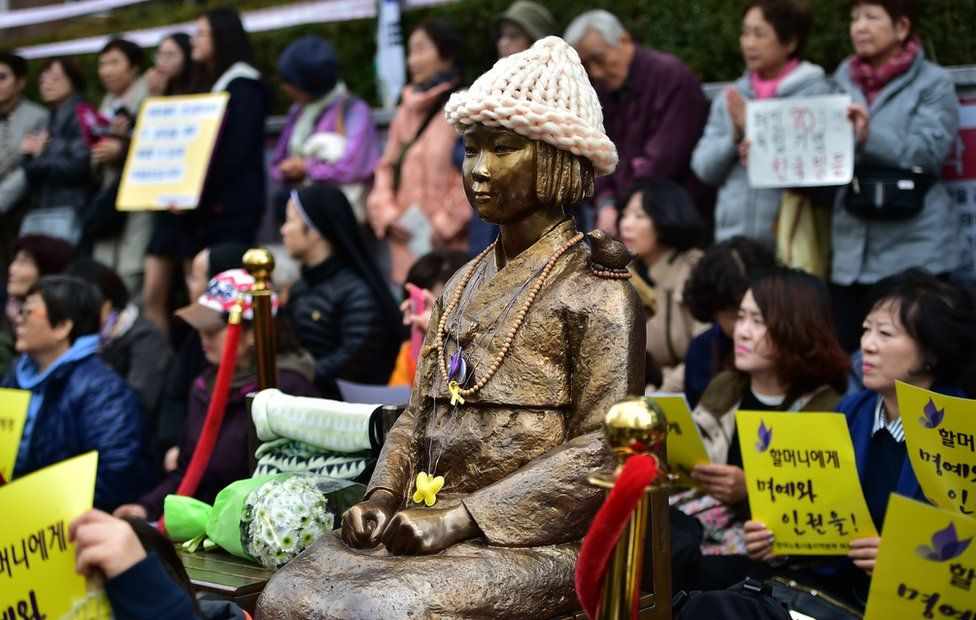
\includegraphics[height = 0.50\linewidth]{/Users/mz/Desktop/GitHub/teaching/gv217_conflict_analysis/figs/wk23/fig1.png}
    \end{center}
    \begin{itemize}
        \pause\item Yet, is China ethnically fractionalized? How can we know?    
    \end{itemize}
\end{frame}

\begin{frame}{Ethnicity}
    \pause Ethnolinguistic Fractionalization (ELF, Alesina et al. 2003, \textit{Journal of Economic Growth})
    \begin{itemize}
        \pause\item \(1 - \Sigma_{i = 1}^{n} s_{i}^2\)
        \pause\item \(s_{i}\) is the share of the group \(i\) (\(i = 1, 2, \ldots, N, \) \(s_{i} \in [0, 1]\))
        \pause\item Malaysia: Bumiputera (60\%), Chinese (20\%), Indian \& Others (20\%)
        \pause      \(ELF_{Malaysia} = 1 - (0.60^2 + 0.20^2 + 0.20^2) = 0.560\)
        \pause\item Singapore: Chinese (75\%), Malay (15\%), Indian \& Others (10\%)
        \pause      \(ELF_{Singapore} = 1 - (0.75^2 + 0.15^2 + 0.10^2) = 0.405\)
    \end{itemize}
\end{frame}

\begin{frame}{Ethnicity}
    \pause Fractionalization \textit{versus} Polarization
    \begin{itemize}
        \pause\item Which polisci field also uses these concepts except conflict?\\
        \pause      The US party system is now highly polarized but not fragmented.\\
        \pause      The opposite is true for some western European countries.
        \pause\item When polarization takes its maximum?\\
        \pause      When there are two groups of equal size
        \pause\item When fractionalization takes its maximum?\\
        \pause      When there are infinitely many equal-sized groups
        \pause\item Which one matters more in conflict analysis?
\end{itemize}
\vfill
\tiny This page's idea was borrowed from Seonghui Lee's GV922.
\end{frame}

\begin{frame}{Ethnicity}
    \pause
    \begin{center}
        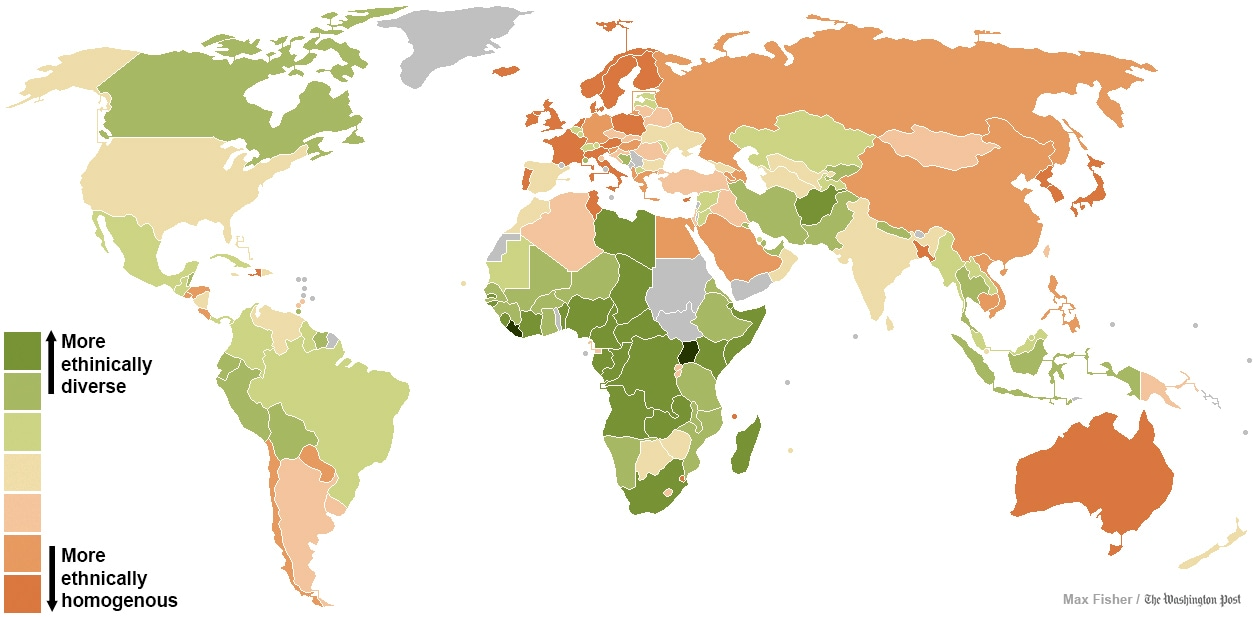
\includegraphics[width = \linewidth]{/Users/mz/Desktop/GitHub/teaching/gv217_conflict_analysis/figs/wk23/fig2.png}
    \end{center}
\end{frame}

\begin{frame}{Examples of Ongoing Ethnic Conflicts}
    \pause
    \begin{center}
        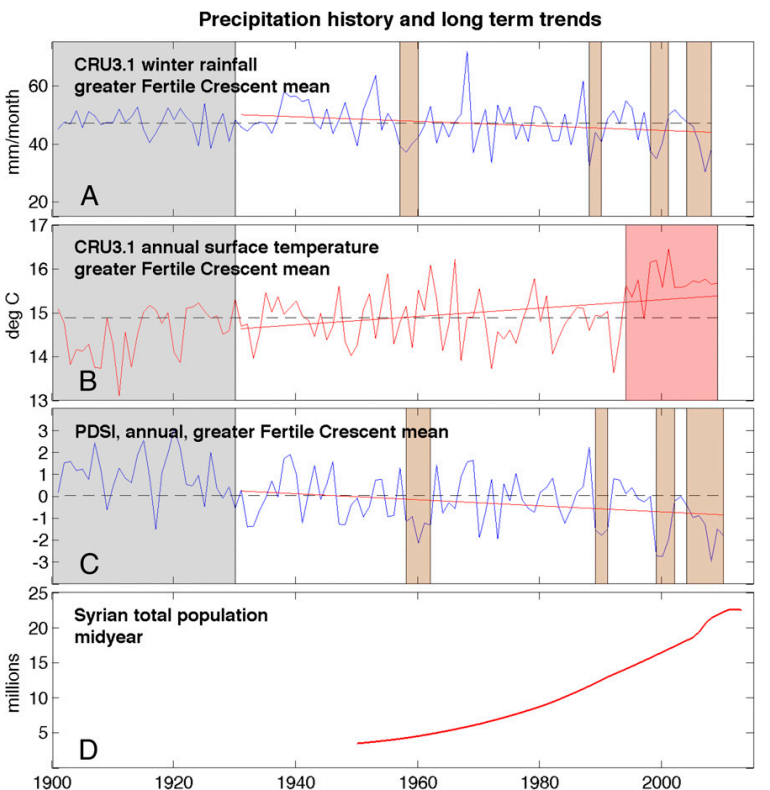
\includegraphics[height = 0.50\linewidth]{/Users/mz/Desktop/GitHub/teaching/gv217_conflict_analysis/figs/wk23/fig3.png}
    \end{center}
    \pause Tigray War
\end{frame}

\begin{frame}{Examples of Ongoing Ethnic Conflicts}
    \pause
    \begin{center}
        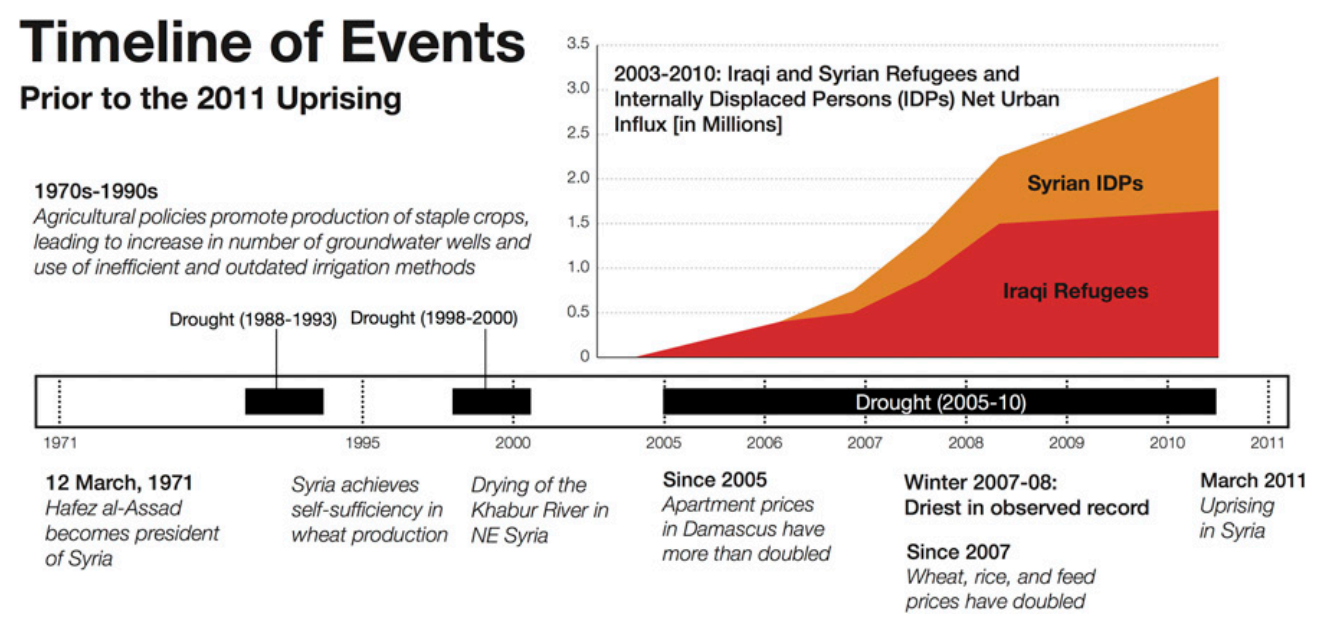
\includegraphics[height = 0.50\linewidth]{/Users/mz/Desktop/GitHub/teaching/gv217_conflict_analysis/figs/wk23/fig4.png}
    \end{center}
    \pause Rohingya Crisis
\end{frame}

\begin{frame}{The Ethnic Origins of Conflict?}
    \begin{itemize}
        \pause\item Ethnic diversity is positively correlated with conflict\\
        \pause      Is it only about ethnic hatred?
        \pause\item Ethnic diversity affects\dots\\
        \pause      inter-personal trust (wk20)\\
        \pause      collective action (wk20)\\
        \pause      \(\Downarrow\)\\
        \pause      public goods provision (wk19)\\
        \pause      economic development (wk19)
    \end{itemize}
\end{frame}

\begin{frame}{Brancati (2006)}
    \pause
    \begin{center}
        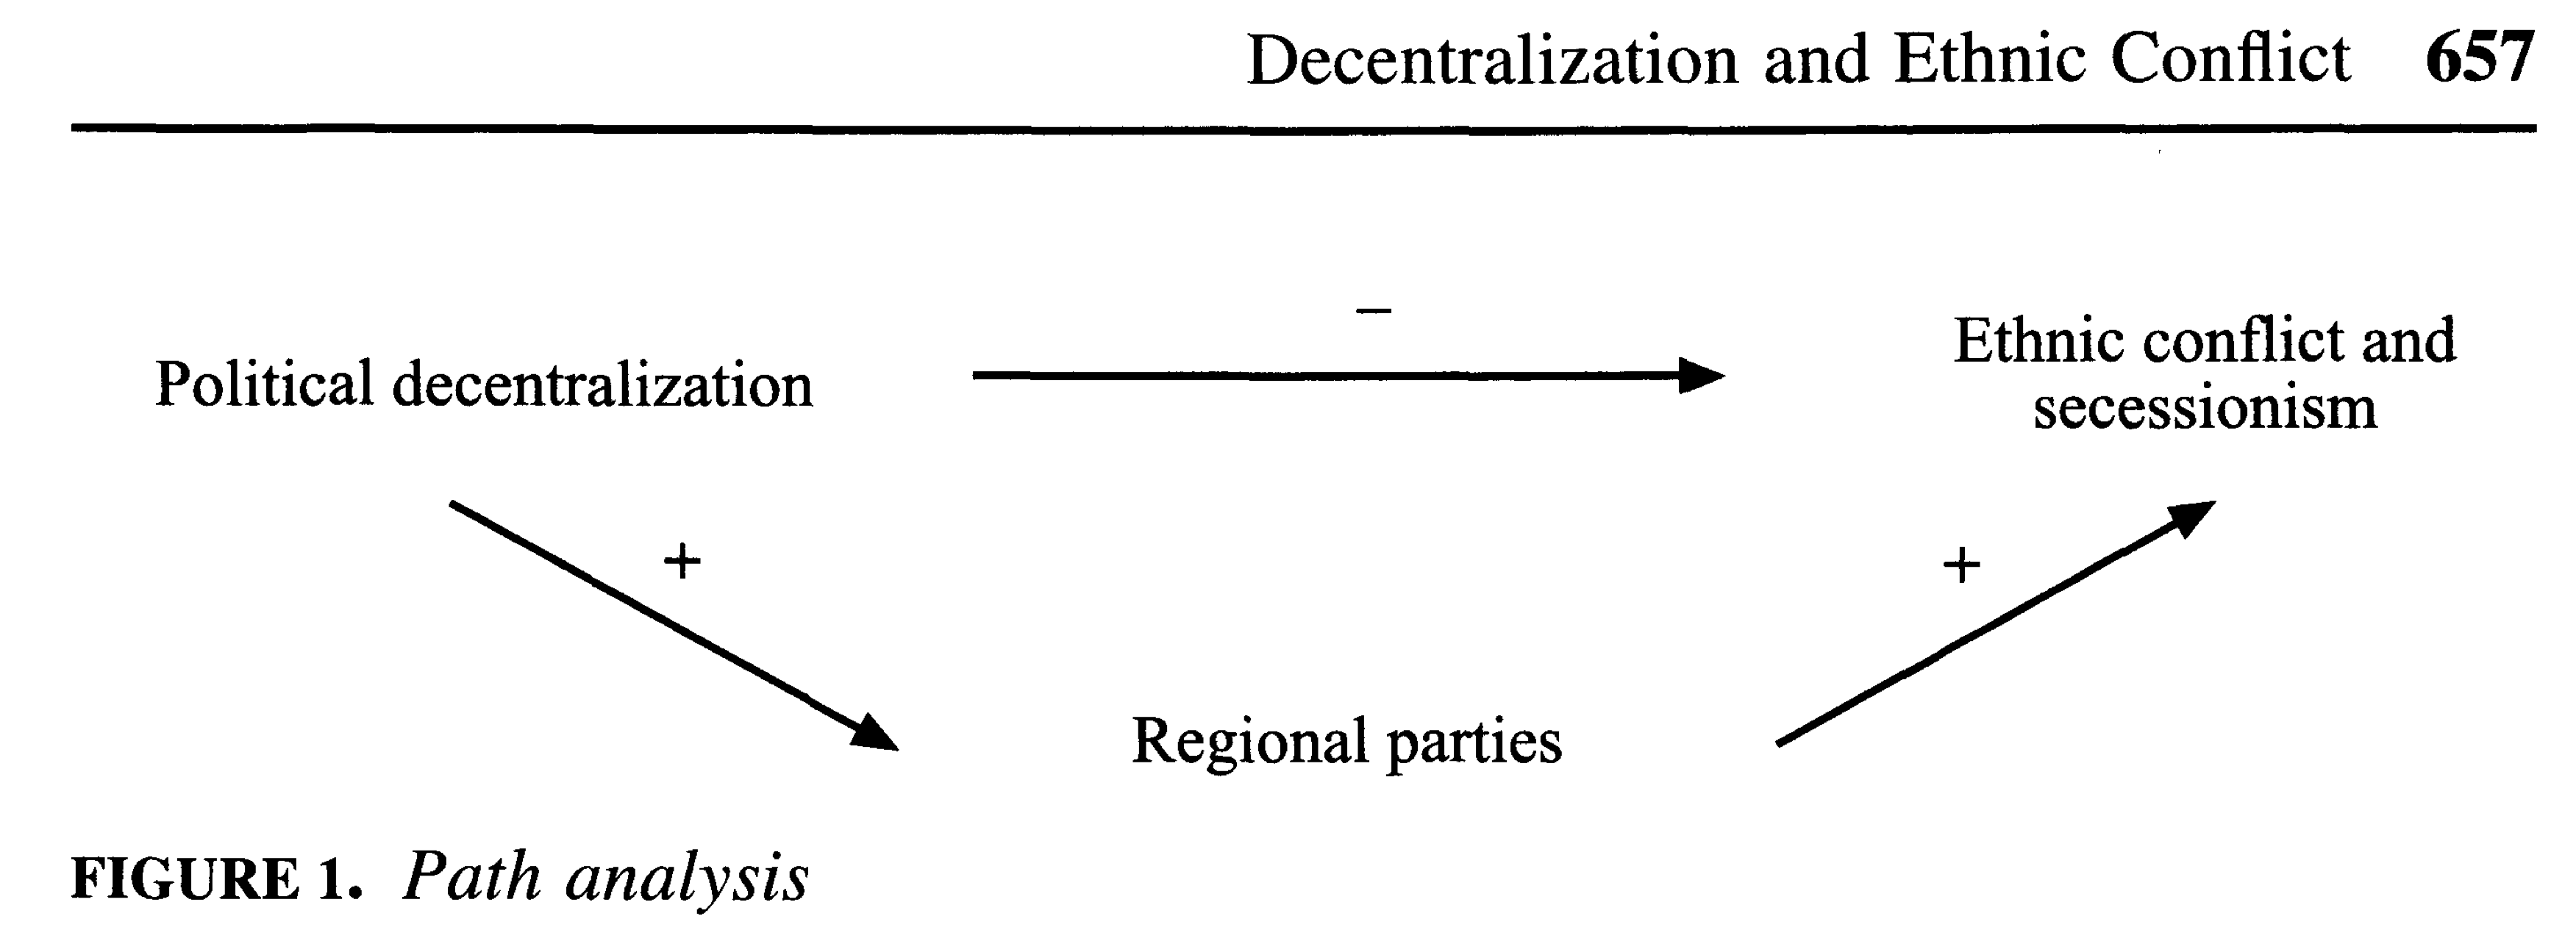
\includegraphics[width = \linewidth]{/Users/mz/Desktop/GitHub/teaching/gv217_conflict_analysis/figs/wk23/fig5.png}
    \end{center}
    \pause Are these arguments causal?
\end{frame}

\begin{frame}{Brancati (2006)}
    \pause
    \begin{center}
        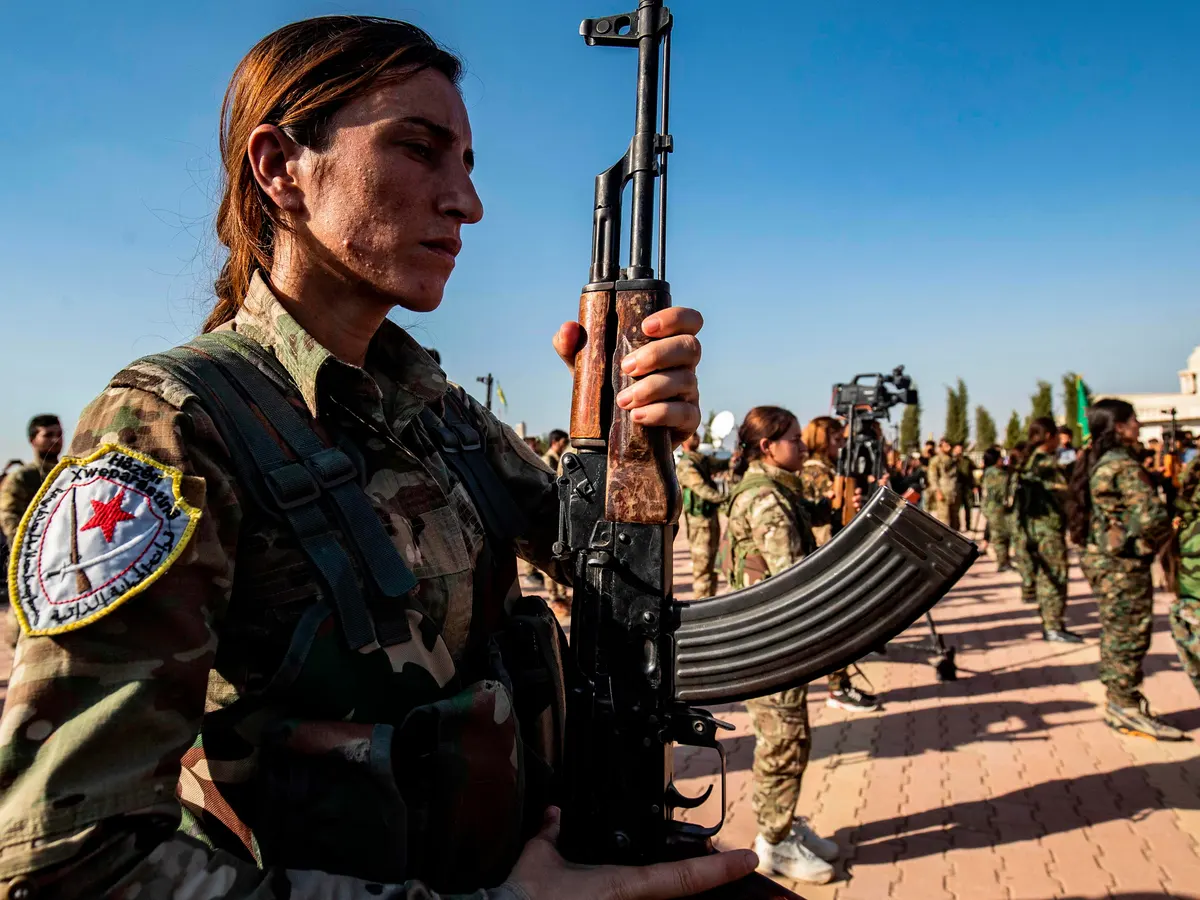
\includegraphics[width = \linewidth]{/Users/mz/Desktop/GitHub/teaching/gv217_conflict_analysis/figs/wk23/fig6.png}
    \end{center}
\end{frame}

\begin{frame}{Brancati (2006)}
    \pause
    \begin{center}
        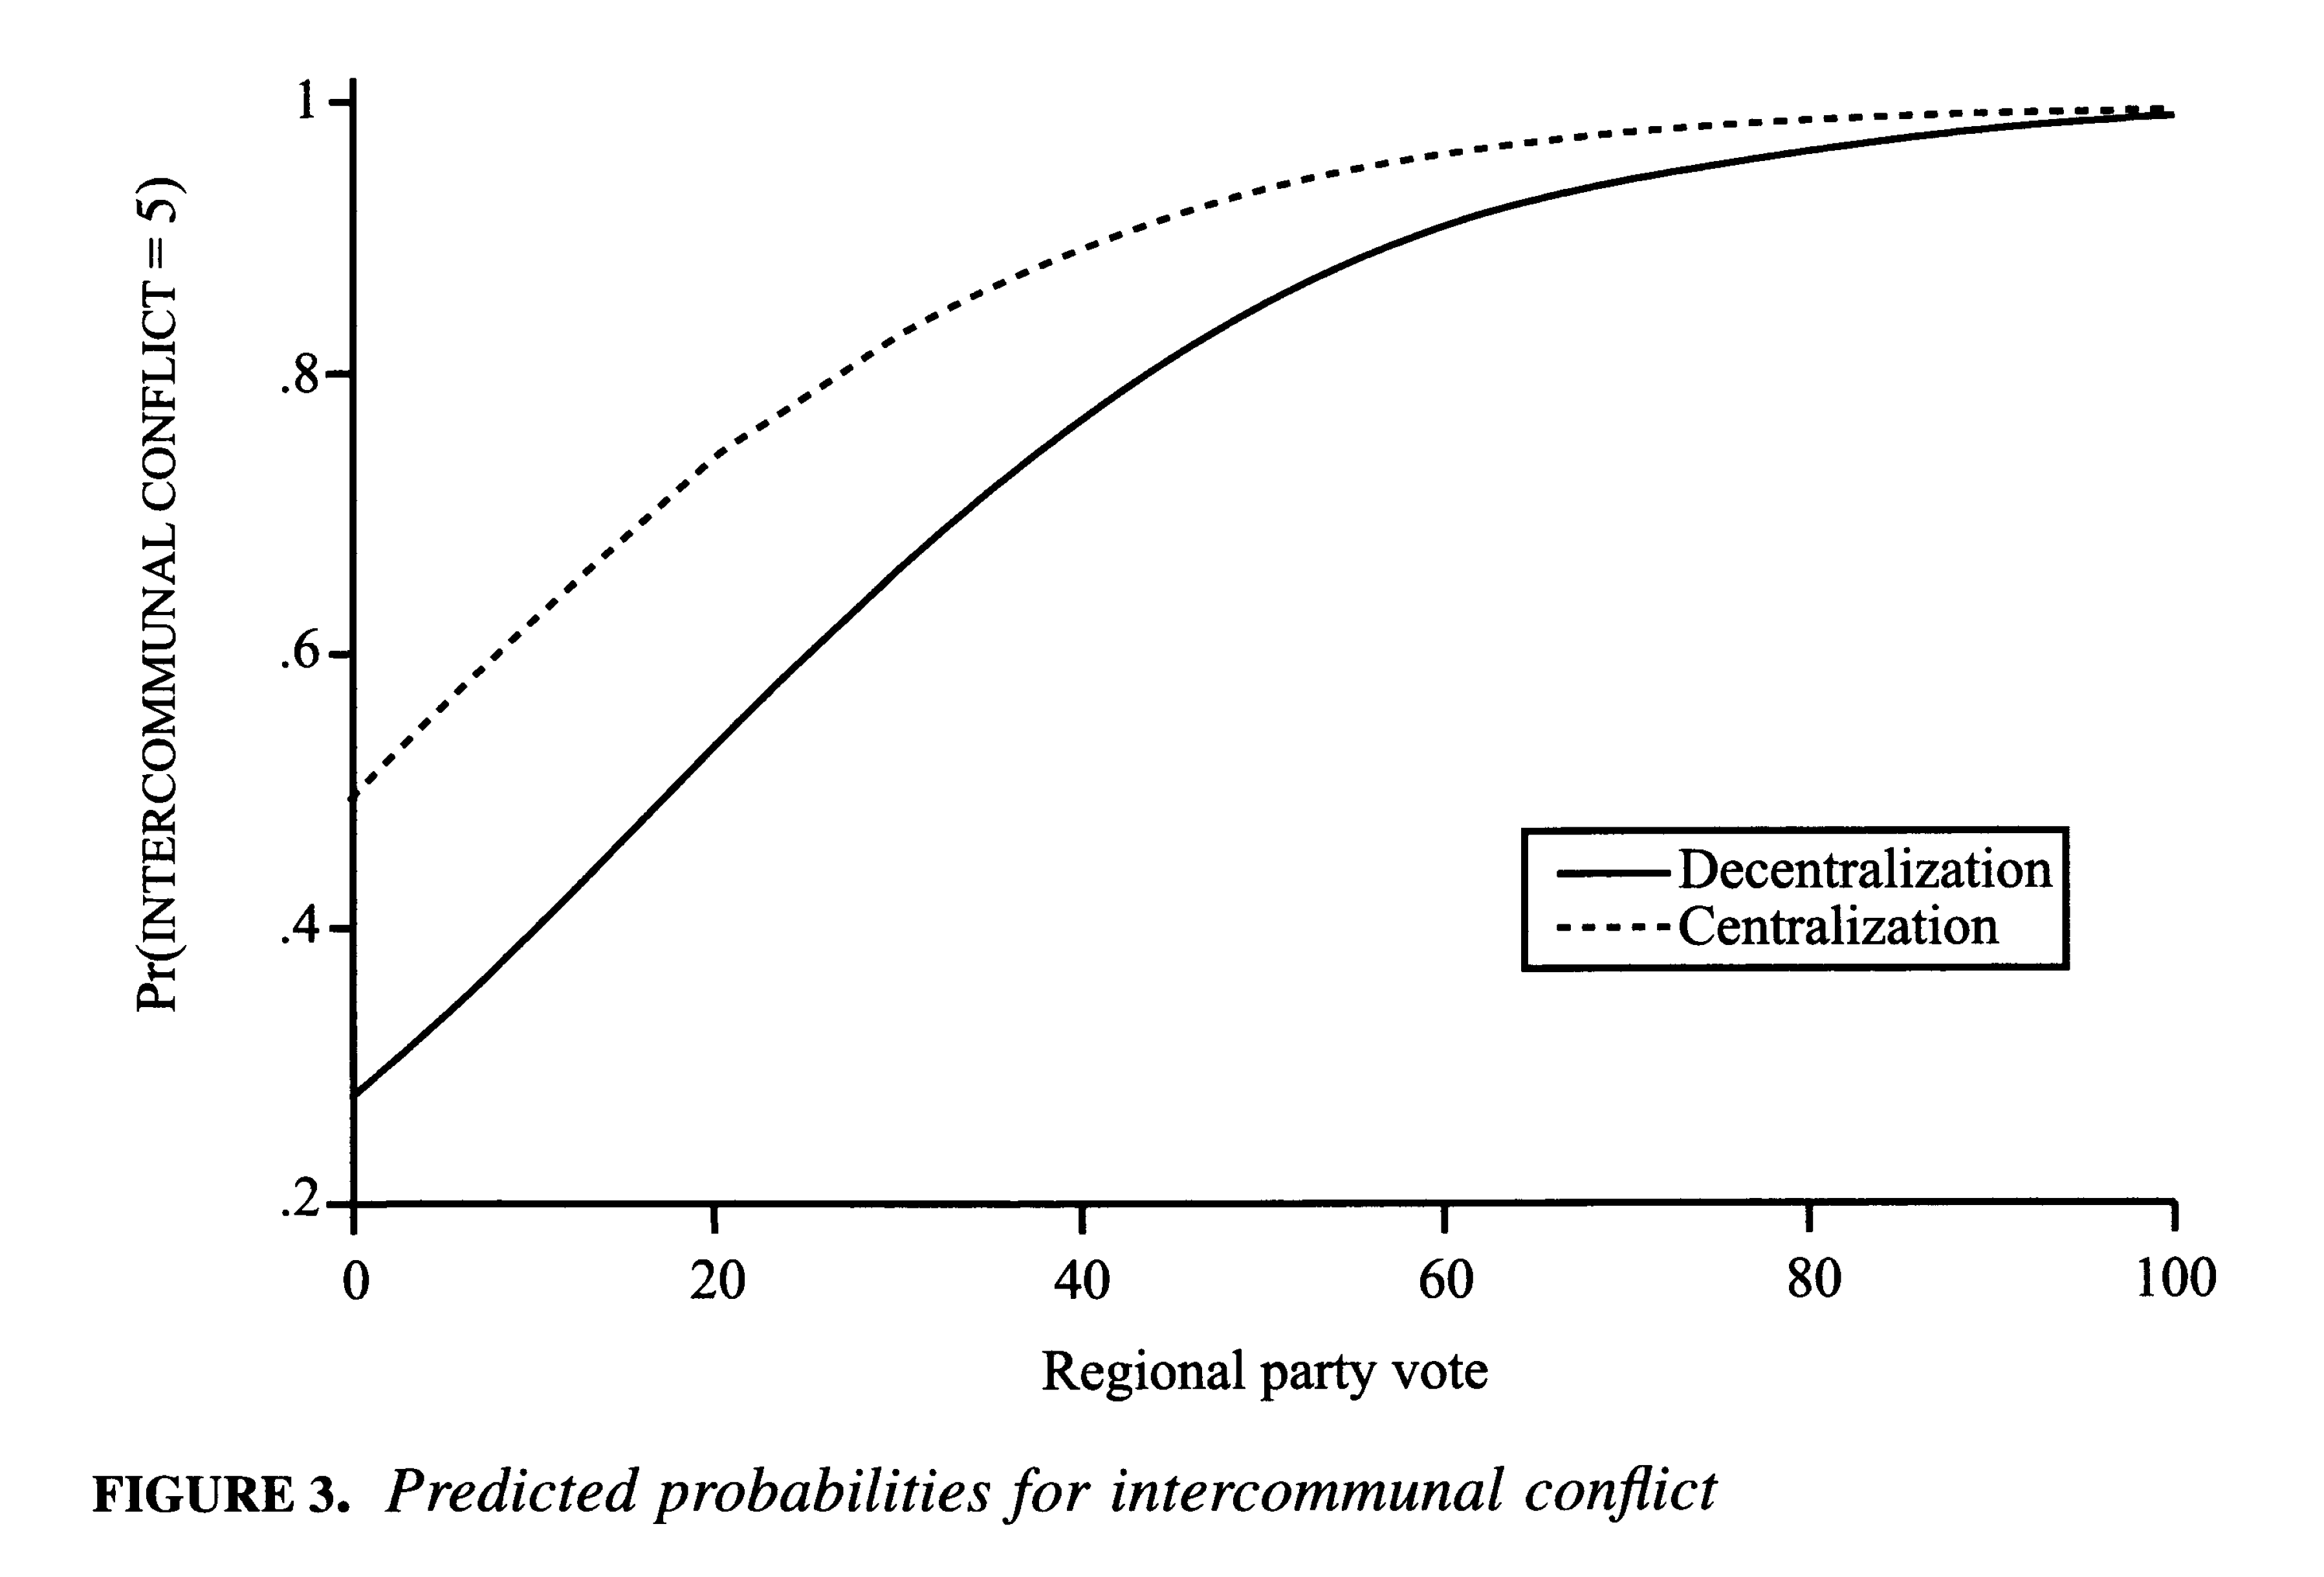
\includegraphics[width = \linewidth]{/Users/mz/Desktop/GitHub/teaching/gv217_conflict_analysis/figs/wk23/fig7.png}
    \end{center}
\end{frame}

\begin{frame}{Cederman, Gleditsch, \& Wucherpfennig (2017)}
    \pause Research question: \pause Whether an increase in governments' accommodative policies toward ethnic groups can plausibly account for a decline in ethnic civil war
\end{frame}

\begin{frame}{Cederman, Gleditsch, \& Wucherpfennig (2017)}
    \pause
    \begin{center}
        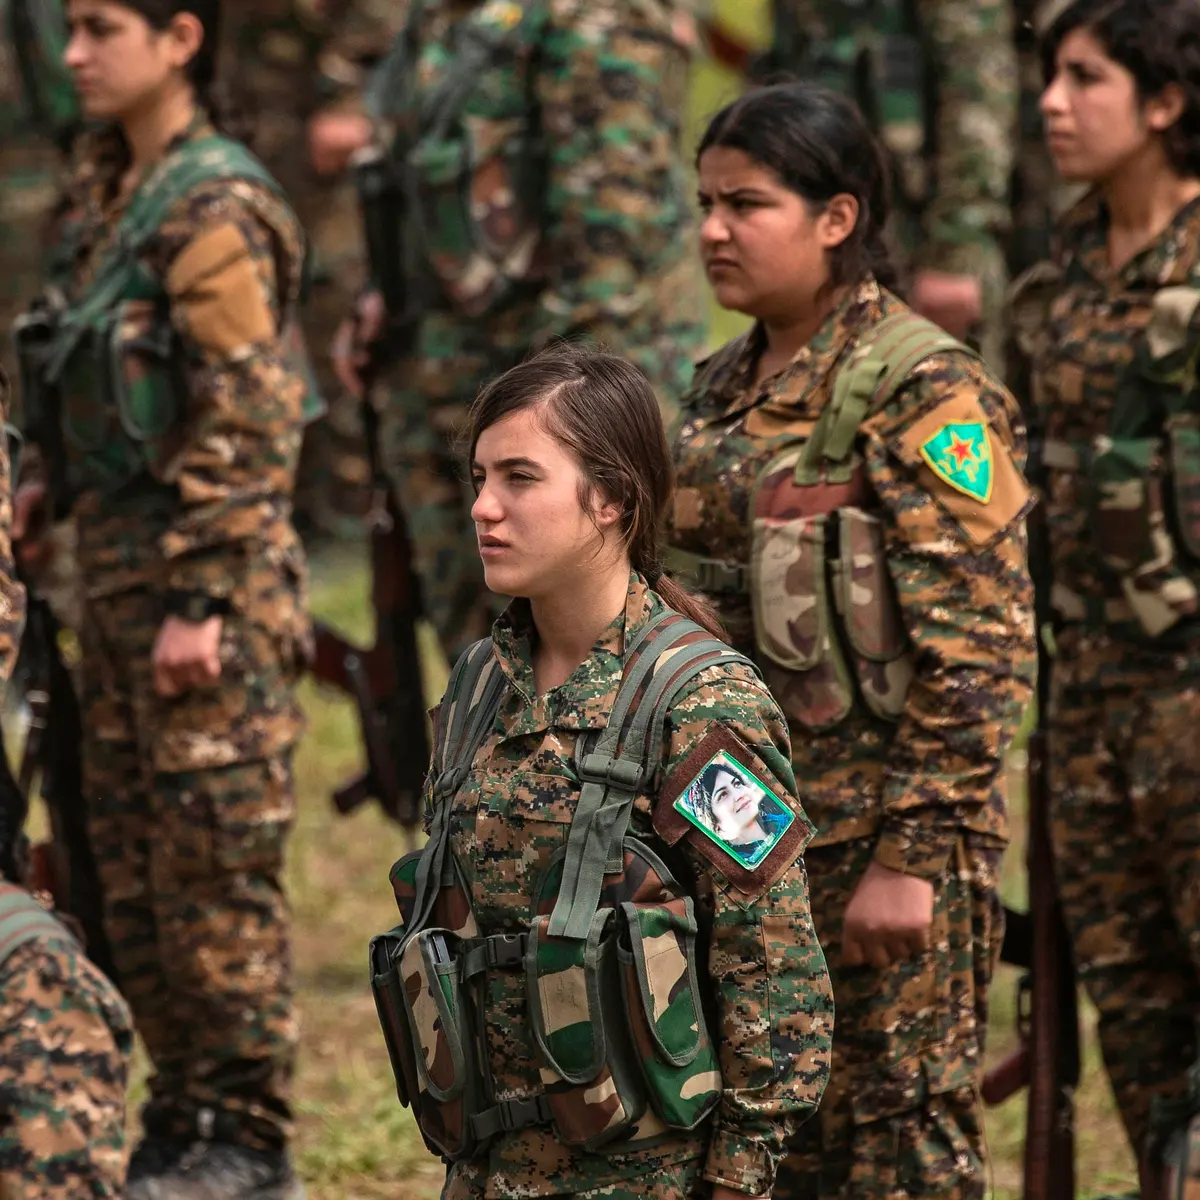
\includegraphics[width = \linewidth]{/Users/mz/Desktop/GitHub/teaching/gv217_conflict_analysis/figs/wk23/fig8.png}
    \end{center}
    \tiny Figure 9. Out-of-sample predictions based on accommodative politics and trend
\end{frame}

\end{document}